%% $RCSfile: using.tex,v $
%% $Revision: 1.1 $
%% $Date: 2010/04/23 01:57:05 $
%% $Author: kevin $
%%
\chapter{Previous and Related Work}\label{C:us}




\section{Related Work}

\subsection{Spatial Auto-Correlation (SPAC)}
Soil liquefaction refers to the process of the saturation of unconsolidated sediments usually by water to the point which the sediments take on liquid like properties. This phenomenon is usually induced during an earthquake event. Sediments, silts and sands below the water table lose their structural strength during an earthquake as they compress the water filled spaces building up pressure to the point that the sediments start to float. At which point the soil layer can no longer support the material above it causing the surface layers to sink \cite{3} \cite{5} \cite{6}.
Spatial Auto-Correlation (SPAC) is a geophysical method that records micro tremors caused by Rayleigh waves to calculate the shear-wave velocity of a stratigraphic column. A low shear wave velocity through a soil layer indicates a very porous material that when submerged below the water table has a high potential to liquefy \cite{2} \cite{7} \cite{10}.

\begin{figure}[h]
\centering
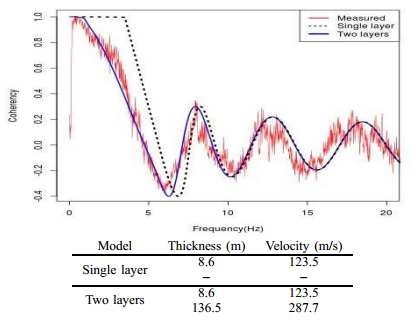
\includegraphics[width=100mm]{simplex.png}
\caption{GP program tree}
\centering
\end{figure}

\subsection{The Computer Programs in Seismology (CPS)}
The Computer Programs in Seismology (CPS) is a software suite containing a number of modules that are able to analyse seismic data like the measured Rayleigh wave data collected using the SPAC method \cite{11}. The suit contains a model of the earths stratigraphic data, specifically, approximate thickness and shear wave velocity data. The modal summation software module calculates a dispersion curve which is then passed to an inversion process, resulting in a theoretical coherency curve which is matched for errors against the data obtained in the field.



\subsection{Simplex Algorithm}
For any linear programming problems the Simplex algorithm is able to deliver a solution. This is the method that is currently used by Geo-technical Engineers in determining the best fit with the theoretical coherency function \cite{2}. The Simplex algorithm with the aid of an operator continuously calls the CPS suit refining the model until no further improvements can be made. It is this process that is slow, time consuming and currently requires heavy human involvement. Figure 2.1 shows a curve being refined with the addition of a second layer.



\subsection{Genetic Programming for Symbolic Regression}
When a model of the curve of best fit is the required objective of a problem you have a regression problem. Therefore as we are using a measured coherency as our target and are creating theoretical coherency curves using the CPS suite we have a regression problem \cite{13} \cite{scoble1}. The accuracy of this theoretical curve against the measured coherency of specific sites is the fitness function for our evolutionary processes.


\subsection{Genetic Programming (GP)}
Genetic programming (GP) is an evolutionary algorithm that given data and a fitness function mutates a function to produce a fitness result. This nature makes it an ideal candidate for regression problems \cite{poli1} \cite{scoble1}. Each evolution of the program is matched against the fitness function and using an elitism technique a subset of the total population is mutated into a new population. Typically a GP programs runs with a tree like structure as can be seen in figure 2.2 \cite{13}. This continues for a predetermined number of cycles and the results of the final elitism selection are returned.

\begin{figure}[h]
\centering
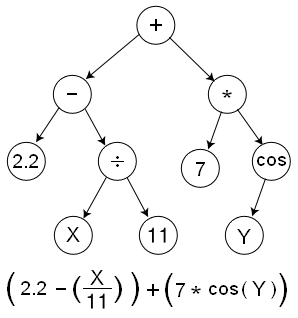
\includegraphics[width=40mm]{Genetic_Program_Tree.png}
\caption{GP program tree}
\centering
\end{figure}



\subsection{Linear Genetic Programming (LGP)}
Linear genetic programming (LGP) is similar in its operation to GP however rather than the tree structures that the GP produces, LGP has a graph based functional structure. This means that previously executed populations are able to be recycled into generations other than their direct children. While this is powerful it does mean minor changes to previous populations can cascade down to younger generations, which can cause large disruptions in the data \cite{poli1} \cite{16} \cite{17}. 


\subsection{Parallel Linear Genetic Programming (PLGP)}
Parallel linear genetic programming (PLGP) limits the dependencies the instructions have between one another. PLGP essentially has a number of LGPs that run separately to one another. Crossovers and mutations are made across the LGPs rather than vertically over themselves. This limits the mutations to equivalent generations. The results is subpopulations that may mutate within themselves but not between populations. Upon completion the final results are added together across the LGPs \cite{15} \cite{22} \cite{23} \cite{24}.


\section{Previous Work}
\subsection{Aaron Scoble's Contribution}

Aaron Scoble successfully implemented the ESPAC system to solve a real world regression task. This achievement was a first and major contribution for PLGP \cite{scoble1}. The problem itself was to create a model that could reliably estimate the liquefaction potential of a specific site during an earthquake event using an autonomous process. The benefits and reasons for this work have previously been outline within Chapter \ref{C:intro}.

Aaron's work used a number of assumptions and simplifications that will be carried over to this project due to the scope. However it needs to be noted that these need to be addressed before any of the techniques can be commercially deployed. The main three are:


 \begin{itemize}
 \item A fixed value of 2 for the number of layers present within each experiment. Aaron suggests a possible solution to this within his work.
 \item The assumption that each of these layers are perfectly horizontal and that no folding or other type of geological deformation has occurred.
 \item The assumption that libCPS and CPS are functioning correctly and are current.
 \end{itemize}
 
 Another major contribution of Aaron's work is the libCPS library that successfully wraps the existing CPS modal summation module into a Java Native Interface (JNI) library \cite{scoble1}. This will be used through each of the Java AI implementations within the project.

